% COS598 Project Paper
% Authors: Aaron Doll, Shaheed Chagani, Michael Kranch, Vaidhyanath Murti
%%%%%%%%%%%%%%%%%%%%%%%%

\documentclass[10pt, letterpaper, twocolumn, twoside]{article}
%\usepackage{epstopdf}
%\usepackage[pdftex]{graphicx}
%\usepackage[left=.8in,top=.8in,right=.8in,bottom=.8in,nohead,nofoot,columnsep=20pt]{geometry}
\usepackage[left=1in,top=1in,right=1in,bottom=1in,columnsep=20pt]{geometry}
\usepackage{setspace}
\usepackage[small,compact]{titlesec}
\usepackage{subfigure}
%\usepackage{multicol}
%\usepackage{multirow}
\usepackage{textcomp}
\usepackage{mathtools}
\usepackage{amsmath}
\usepackage[hyphens]{url}
\usepackage{float}
%\usepackage{fancyhdr}
%\setlength{\headheight}{14.5pt}
%\setlength{\footskip}{11pt}
%\pagestyle{fancy}
%\lhead{}
%\chead{}
%\rhead{}
%\rfoot{}

\newcommand{\tc}{\textcolor}

\makeatletter
\setlength{\@fptop}{0pt}
\makeatother


%make title bold and 14 pt font (Latex default is non-bold, 16 pt)
\title{\bf btctrackr : Something something something}
\author{Aaron Doll, Shaheed Chagani, Michael Kranch, and Vaidhyanath Murti\\
\textit{\{adoll, schagani, mkranch, vmurti\} @cs.princeton.edu}}
\date{COS 598B Privacy \\ 14 May 2014}

\begin{document}

\maketitle

% suppress page numbers
\thispagestyle{empty}

\begin{abstract}
Bitcoin is the mostly widely known and accepted of a rapid growing set of online, virtual crypto-currency. Many users are attracted to these new crypto-currencies because they are decentralized and separated from any sovereignty or authority. They are also adopting crypto-currencies because they provide pseudonymity - an individual can make online transactions with the virtual currency without any direct link to their real world identity. Because of this psuedonymity, many users believe they can use them freely without any risk of their expenditures being traced back to their real identity; however, several recent papers on bitcoin transactions increasingly demonstrate that this belief is false. An individual's spending habits are actually more easily tracked by an unsophisticated advisory due to the public nature of the bitcoin transaction ledger than more commonly accepted online payment methods like credit cards. Continuing on the work presented in ``A Fistful of Bitcoins'' by Meiklejohn et al., this paper revisits the heuristics for identifying an individuals closure, or the subset of linked Bitcoins. We then implement these heuristics in a real-time application made open to the public to allow individuals to avoid linking transactions and monitor the clusters of addresses they wish to transact with. Finally, we discuss several other related projects and future areas for improvement.

\end{abstract}

\section{Introduction}
\label{intro}
In this section, we present a brief overview of technical aspects of Bitcoin. We then describe several known methods of linking Bitcoin addresses presented in previous work. Finally, we discuss issues with these methods and the motivation for a real-time heuristic utility. 

\subsection{Bitcoin}
Bitcoin is an experimental, decentralized digital currency that uses peer-to-peer technology to operate with no central authority. Bitcoins are sent from one address to another with each user potentially having many, many addresses. Each payment transaction is cryptographically signed by the owner to prevent illegitiment spending and then broadcast across the peer-to-peer network to be included in the list of previous transactions (more commonly known as the block chain). Miners are a special type of user that participate in the network. Miners are responsible for verifying the authenticity of an announced transaction based on the previous transactions in the block chain and including that transaction in the next block (update) to the block chain. Once a transaction is included in the block chain, that transaction can not be altered or reversed.

In the Bitcoin protocol, transactions are simply a list of inputs with a corresponding list of transactions as outputs. To generate an address, a user creates a cryptographic key pair with a public and private component. The bitcoin address is an alphanumeric representation of the hash of the public key, while the private key is kept secret and is used to sign transactions to verify their authenticity. Each input is the hash of a previous transaction, as well as an index into the outputs of that transaction, and a script, which is a Bitcoin specific language used for verifying transactions. Each input tuple of (transaction hash, index) is a unique reference to an output of a previous transaction. In order for a transaction to be valid, the sum of all the inputs must be greater than or equal to the sum of all the output address with the difference being claimed by the miner (an optional small fee for publishing the transaction).  Figure \ref{fig:transaction} shows an example transaction where Alice pays Bob 12 BTC. This example also shows Alice paying herself 2.9 Bitcoin into what is commonly called a change address and leaving a transaction fee of 0.1 BTC.

\begin{figure}
  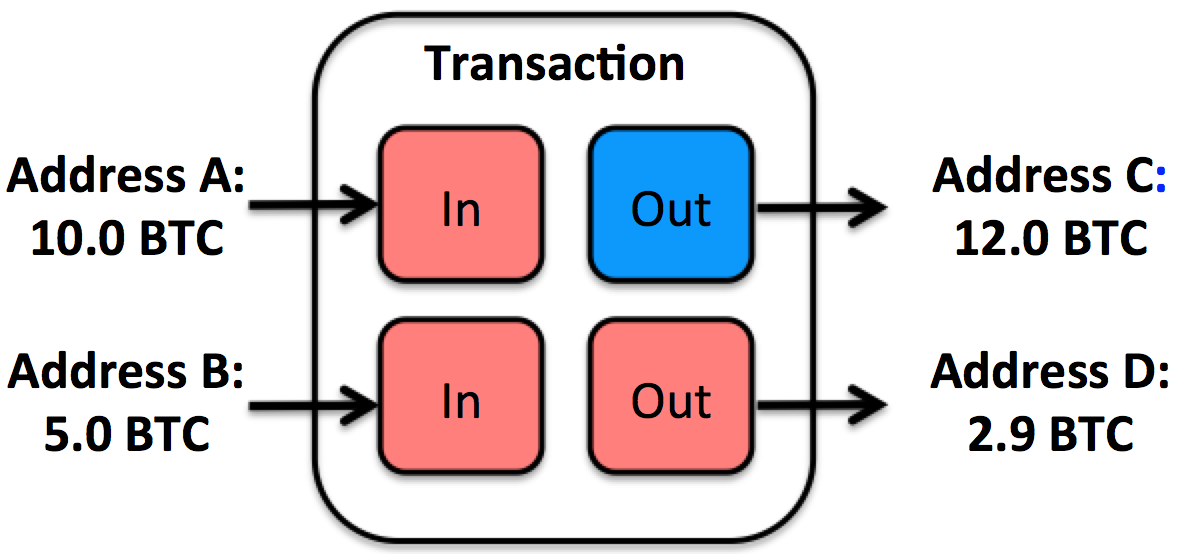
\includegraphics[width=\linewidth]{transaction2.png}
  \caption{Example Transaction}
  \label{fig:transaction}
\end{figure}

\subsection{Address Clustering}

An individual or entity generally controls many addresses as opposed to a traditional system where a user has a single account. The Bitcoin protocol actually recommends using a new address as the output from a previous transaction to increase user privacy, and the vast majority of wallet applications \footnote{Wallets are Bitcoin specific software systems designed to help individual manage their addresses and make transactions} default to generating a new change address in every transaction. In Figure \ref{fig:transaction}, Alice controlled  In this paper, we refer to the term cluster to mean the group (subset) of Bitcoin addresses that are controlled by the same individual. Furthermore, we define control as the individual or set of individuals who possess the private keys that correspond to the addresses in their cluster.

Heuristic one - all inputs below to same user.
Discuss change address - 

\subsection{Motivation}

Users of bitcoin can benefit from a tool that clusters addresses in many ways. First, users are able to monitor addresses that can be linked to them; this makes it easier for users to maintain their privacy. Second, users are able to view the clusters of people they wish to transact with which can help verify the authenticity of the addresses they are transacting with. Finally, users can monitor addresses of special interest in order to estimate the total wealth of certain individuals or organizations (For example, users might wish to monitor addresses that are linked to bitcoin's founder Satoshi). There are few public implementations of this facility and most of them are slow, and sometimes inaccurate.

\section{Related Work}
\label{related}
The initial idea of identifying bitcoin address has been around for quite some time. This idea was first introduced in the original bitcoin paper when noted that you could assume all input addresses belonged to the same individual.

Our system was built as a real-time implementation of the Heuristics described in ``A Fistful of Bitcoins'' by Sarah Meiklejohn et al. 

Bit Iodine is a recently published project out of the . Spagnuolo recently published his project include a front end web service similar our deployment described in this paper.

\section{BTCTrackr}

\subsection{Parser}
When designing our parser, we had two major design goals: we wanted a parser that was incremental, allowing real time updates based on the most recent blocks, and we also wanted to allow users to make nearly instantaneous queries for any address. This ruled out many of the approaches taken by others, such as that taken by Spagnuolo (citation) or Znort987. Both of these approaches used graphs, where connected components are computed on a graph whenever a user makes a query. We decided that this was too slow, so we opted for a database-based approach, where we maintain a database that contains an address-cluster-id mapping. Since blocks are released
approximately every 10 minutes, this allows use to make use of a relatively slow incremental updater using a naive disjoint set implementation. We initially tried this approach for building the database from the beginning, but we quickly realized that this would simply be too slow. After trying a few different data structures, we settled on using a disjoint set maintained in memory, which we wrote to the database after reaching the end of the current chain. At that point we picked up with our incremental, slower database calls. 

Initially, we were going to use a parser written by znort987 (citation!), but after reviewing the code we thought it looked a little unreliable, was slow, and needed some significant changes to accomplish our goals. We started exploring the different bitcoin libraries, and settled on a C++ library called libbitcoin. We primarily chose this library because it looked like it had some solid community support, while also providing some very useful examples and documentation to help us get started. We were also attracted by it's asynchronous event based design. In hindsight, this may not have been the best decision, but it has done an adequate job for the task at hand, with a few exceptions.

In order to find all closures in a block, we iterate through all transactions in the block. For any transactions with more than one input, we attempt to obtain all the input addresses used. This was much harder than we expected, due to what we have assumed to be some irregularities with earlier versions of the bitcoin protocol. In our description of a bitcoin transaction, you may have noticed we made no mention of the addresses of either inputs or outputs. That's because the address is actually contained within the bitcoin script of each input or output. While this is always (?) true for output scripts, we discovered that relying on input scripts containing the address resulted in numerous missing addresses, especially early in the block chain. We aren't sure whether this was a problem with libbitcoin's function for extracting addresses from script or simply the fact it is in an ill-defined format, although we conjecture that this is due to a lack of standardized scripts in the protocol at that time. Fortunately there is another way to get the address, since each input tuple (transaction\_hash, index) uniquely defines an output point of a previous transaction, we can fetch that transaction and extract the address from that output's script. 

This error was in fact related to our biggest problem with libbitcoin: occasional incorrectness. While trying to add balances for each address, we discovered that some of libbitcoin's functions were simply wrong. We narrowed the problem down to missing transactions for some addresses, specifically spends, which lead to massively inflated address balances. After further investigation, we discovered that the problem was the same problem we had in the parser, extracting the input addresses from the script was failing, causing these spends to be left out of queries for the history of specific addresses. We implemented the fix described above, but unfortunately we found there are still transactions missing for select addresses (although much fewer than before). While this doesn't affect our core clustering functionality, it does lead to problems when checking if addresses are linked to each other, causing potential false negatives. By the time we discovered this bug, we had already downloaded the block chain again in order to implement or simple fix, so we didn't have time to investigate further causes of this bug.

\subsection{Database}

After we decided to choose the database approach, we were faced with the decision of choosing an efficient and fast database. We settled on using MySQL for two reasons: First, SQL databases are optimized for queries which tied in well with our goal of providing a fast website. Second, MySQL was easy to connect with both the backend and front-end of our project. We used a simple schema that involved one table with an address as the primary key and an integer that represented the cluster. This set up allowed us to easily insert address-cluster mappings when they were computed by our parser and retrieve the cluster for an address when it was requested by our website. Using MySQL was not without its limitations; it proved to be much slower than we expected while inserting into the database leading to large build cycles. The database insert phase was always the bottleneck in our development cycle, especially given the size of the block chain.

BitIodine, another implementation of this facility, described his setup with 4 separate databases. One holds the block chain, another has the transaction graph, another database contains the balances and other features, and the final one for trades. While this setup might provide more insight into the block chain, we felt that adding more complexity to our setup would result in a increased latency to the website which conflicted with our initial design goals. Because of this, we chose to use just two databases, one fast and lightweight LevelDB database to hold the block chain and the MySQL one that was described above to hold the clusters. We feel that this approach worked well for our purposes.

\subsection{Website}
We designed our web interface with two main goals in mind: we wanted to allow users to ``track'' an address and view detailed information about it, such as which other addresses likely belong to the same entity. Also, we wanted to allow users to enter in two addresses, and see if the clusters containing the two addresses are linked by a transaction. We built our website, www.btctrackr.com, with these goals in mind, and emphasized a simple, clean, easy-to-use design.

Upon visiting our website, the track feature is automatically loaded, in which a user can enter an address and press "Track". We send an AJAX request to our server, which looks up the $cluster\_id$ of the address in our database, and then retrieves all of the addresses corresponding to that $cluster\_id$. There are a number of front-end and backend checks we have in place to ensure the user has a valid Bitcoin address. On the client side, we make sure the address is a valid number of characters. On the server side, if the address is not present in our database, we query the blockr.io API to check if the address has ever appeared in a transaction, whether or not it is valid. If it is not valid, we alert our users accordingly.

We also wanted to display the current balance of each of the addresses, as well as the total balance of the entire cluster. Due to problems with the libbitcoin library, we chose to leverage the blockr.io API, which has up-to-date balance information. Once challenge we faced, however, is that querying a web API is for several balances is way slower than querying a local database. Some of our clusters have hundreds or even thousands of addresses, and making this many API calls would lead to a tremendous delay in response time for the users. Our goal was to make our interface as seamless and snappy as possible, so we spent time devising a solution to the problem. The blockr.io API allows clients to get balance information for up to 20 addresses in one call, so after retrieving all of the cluster addresses from the database, we grouped them into sets of 20 or less. Then, we utilized $curl\_multi\_init()$ (through the parallelcurl Github library) to send off all of these API calls simultaneously, and process the results asynchronously. We found that we were able to return results to the user way faster than if we used any other method. For example, we are able to return over 100 balances in less than 1 second. The user interface is very responsive, which makes our tool easy to use.

[Talk about shortest path here, once it is properly implemented]

\section{Evaluation}

\section{Future Work}
Our project does have some limitations, many of them due to our use of libbitcoin. Libbitcoin does not support multi-signature transactions as of yet, limiting the transactions we include in our cluster calculations. As we mentioned earlier, we have noticed some missing transactions, leading to potential false negatives when we check for one hop links between clusters. We hope that this is related to the earlier problem and primarily happens for early addresses, but since we wouldn't be able to update our data at this point even if we do find the bug, we have left this for a future date. 

There are also a number of features that we simply couldn't include due to time constraints. In ``A Fistful of Bitcoins'', the authors associate clusters with entities and graph the largest entities. We wanted to include the ability for users to submit labels to addresses, hopefully mapping the bitcoin network in detail, as well as including addresses that we labeled ourselves. One feature that we wish we had implemented is arbitrary length shortest paths, but we figured that it wasn't worth the extra time to implement if we couldn't be sure of its accuracy. In our first conception of this project, we also hoped to implement the change address heuristic, but after speaking with Meiklejohn, we decided that wasn't a realistic goal for a semester long project.

\section{Conclusion}

% Imports the bibliography, don't remove
\small{
\begin{thebibliography}{99}

\bibitem{libbitcoin} Maersk, N., Strateman, P., Taaki, A., and Williamson, R., ``libbitcoin - Asynchronous C++ Bitcoin library'', \emph{GitHub Repository,} 2013,
\url{http://libbitcoin.dyne.org/}.

\bibitem{fistfull} Meiklejohn, S., Pomarole, M., Jordan, G., Levchenko, K., McCoy,
D., Voelker, G. M., and Savage, S., ``A Fistful of Bitcoins: Characterizing Payments Among
Men with No Names,'' in \emph{Proceedings of the 2013 Internet Measurement Conference,} 2013, \url{http://cseweb.ucsd.edu/~smeiklejohn/files/imc13.pdf}.

\bibitem{bitcoin} Nakamoto, Satoshi, ``Bitcoin: A Peer-to-Peer Electronic Cash System,'' (2008) \url{https://bitcoin.org/bitcoin.pdf}.

\bibitem{bitiodine} Spagnuolo, Michele, ``BitIodine: Extracting Intelligence from the Bitcoin Network (Master's Thesis),' 2013, \url{https://bitiodine.net/}. 

\bibitem{znort} Znort987, ``Block Parser'', \emph{GitHub Repository,} 2012,
\url{https://github.com/znort987/blockparser}.



%P.W.D. Charles, Project Title, (2013), GitHub repository, https://github.com/charlespwd/project-title

\end{thebibliography}
}
%Bit Iodine - http://miki.it/articles/papers/#bitiodine
%Fistful of Bitcoins - cseweb.ucsd.edu/~smeiklejohn/files/imc13.pdf


\end{document}